% Chapter Template

\chapter{Design and Development} % Main chapter title

\label{DesignAndDevelopment} % Change X to a consecutive number; for referencing this chapter elsewhere, use \ref{ChapterX}

\lhead{Chapter \ref{DesignAndDevelopment}. \emph{Design and Development}} % Change X to a consecutive number; this is for the header on each page - perhaps a shortened title

%----------------------------------------------------------------------------------------
%	SECTION 1
%----------------------------------------------------------------------------------------

\section{The design of \theartefact}
%%%%%%%%%%%%%%%%%%%%%%%%%%%%%%%%%%%%%%%%%%%%%%%%%%%%%%%%%%%%%%%%%%%%%%%%%%%%%%%%%%%%%%%%%
%%%%%%%%%%%%%%%%%%%%%%%%%%%%%%%%%%%%%%% TODO %%%%%%%%%%%%%%%%%%%%%%%%%%%%%%%%%%%%%%%%%%%%
%%%%%%%%%%						Intro to section							%%%%%%%%%%%%%
%%%%%%%%%%%%%%%%%%%%%%%%%%%%%%%%%%%%%%%%%%%%%%%%%%%%%%%%%%%%%%%%%%%%%%%%%%%%%%%%%%%%%%%%%

\subsection{Design}
The artefact was divided into several modules which function independently of each other.
The modules were loosely coupled so that each module could be changed or modified without affecting the other modules.
The modules that were created were:
\begin{itemize}
	\item The web front end
	\item A module that fetched and processed the HTML from the sites that the user wanted to mark up
	\item A module for fetching possible disambiguating terms from lexitags
	\item A module for finding the best fit mappings for SUMO and schema.org
	\item A module for finding the best fit mappings from DBPedia to schema.org
	\item A module that puts the document back in its initial state and saves it to a persisten storage
\end{itemize}

\section{Run through of common use}
Common use case:
User comes to site -> Basic site generated from template on server

The user enters URL of page to tag:
\begin{itemize}
	\item URL gets sent to proxy module on server
	\item Proxy fetches the HTML of the target URL
	\item Proxy comments out script and iframe tags
	\item Proxy replaces relative image URIs with absolute image URIs.
	\item Proxy sends back an object containing the sites head and body tag
	\item The content of the body tag is used to populate the content container in the web app.
\end{itemize}
The user highlights a word on the page to add meta data to:
\begin{itemize}
	\item The text of the highlighted selection gets sent to the lexitags server for disambiguation
	\item The results from lexitags are filtered
	\begin{itemize}
		\item If the results contain WordNet terms, then the DBPedia results are filtered away
	\end{itemize}
	\item The results are then sorted
	\begin{itemize}
		\item Primarily by source, WordNet terms first, then the first and second level schema.org terms
		\item Secondarily they are sorted lexically
	\end{itemize}
	\item Then the results are displayed on the web page. If the user cannot find a match with the highlighted text,
	it is posible to write your own word into a search box.
	The semantics of this word will then be linked to the highlighted text.
\end{itemize}
The user click the sense of the word which match the intended semantics of the highlighted word
\begin{itemize}
	\item The term, either a WN synset or a DBP entity gets sent to the mapping module on the server
	\item The mapping module find the mappings into other ontologies
		that most closely matches the semantics of the term.
	\item The server returns the entity types that best fit the term, and their namespaces
		\item If no schema.org mapping is found, schema:Thing is returned as it is always correct.
	\item The web app adds a tag which surrounds the selected text, and adds the entity value to it using RDFa
		\item This new tag contains keywords which will highlight it on the page
	\item The web app then asks the server for the schema.org properties of it's schema type(s).
	\item The server returns all the applicable properties
	\item The web app adds all the returned properties to the markup of the page with empty values
\end{itemize}
The user clicks a marked up section
\begin{itemize}
	\item The web app displays all the possible attributes the section can have
	\begin{itemize}
		\item If values have already been inserted, these are shown as the default values
	\end{itemize}
	\item The user inputs the values the attributes should have
	\item When the submit button is click, the attributes get updated to the correct values
\end{itemize}
The user clicks the export button
\begin{itemize}
	\item The html on the page is cleaned
	\begin{itemize}
		\item Temporary markup(tooltips, popover) is removed
		\item Attributes without values are removed
	\end{itemize}
	\item The html is sent to the server
	\begin{itemize}
		\item The exporter comments in the script and iframe tags
		\item The html is put in the database
	\end{itemize}
	\item The server returns the id of the new web page
	\item The web app displays the URL to the new marked up website.
\end{itemize}
\subsection{Designing the algorithms}
We will now describe the two algorithms that were developed to find mappings between the WordNet synsets and the ontologies.
We use two axes for navigating the WordNet graph, the hypernymes and the hyponymes.
As described in \ref{TheoryWordNet}, a hypernyme can be described as category words into which more specialized words fall.
Hyponyme is the inverse relation, where a hyponyme is a word which can be generalized into some more general category.
For simplicity we will also use one additional term.
We will use \emph{sibling} to refere to words which are hyponymes of a words hypernyme.
An example( see figure \ref{Hyponyme}, page \pageref{Hyponyme})
would be that \{dog\} has the hypernyme \{domestic\_animal\}, which again have the hyponyme \{cat\},
\{cat\} would then be considered a sibling term of \{dog\}.


Our hopes for this mapping tree is that in the cases where there is no direct mapping from the synset to a term in the
ontologies we are mapping to, we can always preserve the semantics of the synset by using one of the synsets ancestors.
For the siblings we hope that if we find a mapping,
then the parent term of the term we have mapped to in the ontology will correspond to the meaning of the synset.
Both these propositions will be tested as a part of the work with the thesis.

The algorithms define different orders of looking at the synsets

\subsubsection{Generating the search tree}
The first step of the algorithm is the same for both algorithms.
A search tree is generated using a perl script
\footnote{Perl script found at \url{https://raw.github.com/EivindEE/SemTag/master/scripts/parents.pl}.}.

\begin{figure}[h]
    \begin{center}
        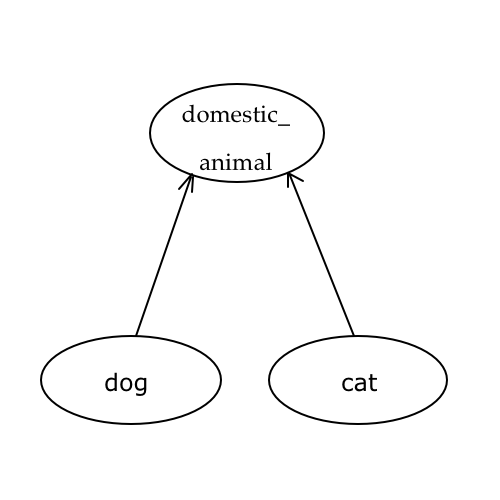
\includegraphics[width=0.60\textwidth]{Hyponyme_own.png}
        \caption{The hyponyme relation, modified from \protect \citet{Miller1990}}
        \label{Hyponyme}
    \end{center}
\end{figure}



\subsubsection{The sibling first algorithm}
The sibling first algorithm traverses the search tree by first looking if there is a direct mapping from the base synset to the ontologies.
If a direct mapping is not found, it will look at the hypernyms and see if it has a mapping.
After looking at the hypernyms it will look at the sibling senses.
It will then go on to look at the hypernyms of the hypernyms, and then their sibling states.
It will continue to follow the hypernym chain upwards until there are no more hypernyms, or a mappings has been found.

\subsubsection{The ancestors first algorithm}
The ancestor first algorithm will follow the hypernym chain upwards looking for mappings.
The algorithm is written to follow the hypernym chain again, looking at the sibling senses, if no mapping is found.
But since every WordNet noun is a hyponyme of {entity}, which should map to the most general object in an ontology,
it will likely never be touched.


%----------------------------------------------------------------------------------------
%	SECTION 2
%----------------------------------------------------------------------------------------

\section{The development process}


\subsection{Iteration 1}
The first iteration started with getting to know the technologies, and setting up a framework
Quite some time was spent getting comfortable working with the \nom{DOM}
{The Document Object model, convention for interacting with HTML elements},
and the peculiarities of the different mainstream browsers.
At this point we also set up the server that the web app would run on.

\subsubsection{Server setup}
Setting up a basic server in node.js can be done in a single line of code,
but requires a lot of low level handeling of requests and responses
including parsing request url to find the correct handler.
We decided to instead go for express\footnote{\url{http://expressjs.com}},
a web app framework which simplifies routing requests to the correct handler and handeling static files.
%Additional benefits of using the framework included simplified logging of requests, and
It was also decided to use the jade\footnote{\url{http://jade-lang.com}}
templating language to generate the \nom{HTML}{HyperText Markup Language} that was used on the website.
Using a templating language made the distinction between structure and content clearer,
and enabled reuse of structure and content between different versions of the website during development.


\subsubsection{Representing other websites}
One of the issues that come up early was how to display the websites that the user wanted to add metadata to.
Early attempts tried using the iframe\footnote{http://www.w3.org/TR/html5/embedded-content-0.html\#the-iframe-element}
element of \nom{HTML}{HyperText Markup Language}.
Embedding the target website in an iframe was the first try as it would allow the page to display in the same maner
as it does when accessed directly.
Using the iframe element in this maner would however constitute cross-domain communication and is not allowed.

This problem was not solved in the first iteration.
After trying to find a workaround it was decided that displaying html from other websites was not essential to the work,
and that the focus should be shifted to adding markup.
The solution we landed on was to insert some placeholder text which was used for testing purposes.
This placeholder text is still displayed on the website to give visitors something to try the tool on before using it
to add markup to their own pages.

\subsubsection{Interaction method}


\subsection{Creating the mapping files}
An important part of the early work was to generate files that the tool could use to find mappings from WordNet synsets
into the ontologies which were used.
The ontologies that were chosen for the project, SUMO  and schema.org, already had these kinds of mapping files.
The mapping files were however in different formats and inn formats that were unsuitable for use in a javascript based application.
The format we wanted was one that gave up the option to ask if there was a mapping for a given WordNet synset,
inn other words what we wanted was a dictionary.
Javascript objects are themselves dictionaries, making it natural to choose to them as the representation.
The structure of the objects is very simple, the synsets are used as the keys to entities in the target ontologies:
\begin{lstlisting}[caption=Excerpt from the \href{https://github.com/EivindEE/Madame/blob/master/mappings/wn2schema.js}{wn2schema.js} mapping file]
exports.mapping = {
	"abstraction#n#6": "Intangible",
	"accounting_firm#n#1": "AccountingService",
	"address#n#6": "PostalAddress",
	// The rest of the mappings
	"work_unit#n#1": "Energy"
};
\end{lstlisting}

Since we use javascript objects to represent the mappings, querying a mapping object to check if it contains a mapping for a certain synset would then just consist of checking if
the object has a property with the given name:
\begin{lstlisting}[caption=Testing if a mapping exists]
    if (mapping['synset-to-check']) {
        // it contains a mapping
    } else {
        // it does not contain a mapping
    }
\end{lstlisting}

The mapping files were to large to translate to javascript objects by hand, with the SUMO mapping file alone
covering more than 82.000 mappings, so we used regular expressions to modify the files globaly.
The schema.org mapping file\footnote{\url{https://github.com/mhausenblas/schema-org-rdf}}
that was used as the basis for the wn2schema mapping file is written inn \nom{RDF/XML}{An XML representation of RDF}.
The first step in creating the mapping file was to remove the parts of the file that were irrelevant to the problem at hand.
The original file contains triples describing schema.org properties,
the schema.org entities and the hierarchal ordering of entities.
This information is handled at other places in the tool we are creating and could be safely removed.
Only the elements mapping synsets to schema.org terms were kept, and all other information except the names were removed.
At this point the XML tags were stripped so only the synset reference and the schema type remained.
Since we now had the correct elements in the correct place we needed only to surround them with the correct quotation
marks, separate them with a colon and add a comma at the end to separate it from the next property.

The SUMO\footnote{\url{http://sigmakee.cvs.sourceforge.net/sigmakee/KBs/WordNetMappings/}} mapping followed a similar pattern,
but the original format was different as it used the WordNet database format.
We used the WordNetMappings30-noun file as our basis so for this mapping we did not have to remove non noun phrases.
The fact that each line in the file corresponded to a line in the mapping file made the process of translation easier,
there was however one caveat in that the file used the offset to identify the synset,
instead of the normal word\#category\#number which we use.
We put some work into finding a way of substituting the offset for the synset id,
but found that it was simpler to find the offset for the synsets that were queried.
-- Unifying the way the properties are named is one of the things that can simplify the generalization of the process at a later stage.


%% Trying Perl syntax
\begin{lstlisting}[language=perl, caption=experiment]
my @parents = parent($synset);
my @all_parents;
while ( @parents){
	my $parent = shift @parents;
	push(@parents, parent($parent));
	push(@all_parents, $parent);
}

my @all_parents_with_siblings;
push(@all_parents_with_siblings, {"synset" => $_ , "offset" => $wn->offset($_) ,"siblings" => [siblings($_)]}) for @all_parents;

my %json = ("chain" => [uniq(@all_parents_with_siblings)], "synset" => $synset, "offset"=> $wn->offset($synset), "siblings" => [siblings($synset)]);
my $json = JSON->new->utf8->pretty->encode(\%json);
print $json;

sub parent {
	my @parents = $wn->querySense($_[0], "hype");
	if ($#parents > 0) {
		return ();
	}
	return @parents;
}

sub siblings {
	my $synset = $_[0];
	my @parents = parent($synset); # Find parents of synset
	my @siblings;
	my @sibling_and_offset;
	push(@siblings, $wn->querySense($_, "hypo")) for @parents;
	my $index = 0;
	for my $value (@siblings) { # Removes term from siblings
		if ($value eq $synset) {
			splice @siblings, $index, 1;
		}
		$index += 1;
	}
	for my $sibling (@siblings) {
		push (@sibling_and_offset, {"synset" => $sibling, "offset" => $wn->offset($sibling)});
	}
	return @sibling_and_offset;
}
\end{lstlisting}
